%!TEX root = ../../Master.tex
\section{Algorithms for pathfinding}
Graph Search Algorithms analyses the structure of a graph. This can be used to find the shortest path from one vertex to another, in a graph \cite{Cormen2009}. Some graph search algorithms are more efficient than others, at finding the shortest path connecting two vertices in a graph.

Finding the shortest path from one vertex to another, is defined as a single-pair shortest path (SPSP) problem. Finding the shortest path from a single source vertex to all other vertices, is defined as a Single Source Shortest Path (SSSP) problem.


This section describes both Dijkstra's algorithm , which is used for solving SSSP problems, in \cref{subs_dijkstra}, and the A* algorithm, which is used for solving SPSP problems, in \cref{subs_astar}. These algorithms are very alike, but they each differ in a few important ways. They will both always find the shortest path, however Dijkstra's is inefficient in terms of speed, while the A* algorithm is dependent on an admissible heuristic. This is explained in \cref{subs_astar}.

%   In \cref{sec:specification} we specified that our solution needs to find the shortest weighted path to the destination.
%   To better understanding pathfinding we examined different algorithms. We discovered that some algorithms have a high accuracy but is slow at finding the path, and conversely.
%   We have compared some well known path finding algorithms by evaluating their calculation time and route precision.

%   In the following we compare 3 frequently used algorithms:
%   \begin{itemize}
%     \setlength{\itemsep}{1pt}
%     \setlength{\parskip}{0pt}
%     \setlength{\parsep}{0pt}
%     \item \textbf{Dijkstra's Algorithm} Always finds the shortest path but has long calculation time on more complex graphs.
%     \item \textbf{Greedy Best-First-Searches} Is a very fast algorithm but does not always find the shortest path.
%     \item \textbf{A* Algorithm} Is an extension of Dijkstra's Algorithm but has less calculation time using heuristic values.
% \end{itemize}

% The A* algorithm was chosen as the algoritm of choice because it always finds the shortest path, and still has a reasonable fast computing time. This algorithm also makes it easier to implement stairs and elevators, because of the heuristic values. In this section we will describe A* and Dijkstra's because A* is an extension of Dijkstra's.


  %Path finding algorithms are used for finding a path between two locations, the source and the destination. By searching its way from the source to the destination, until a path is found. These algorithms also make it possible to calculate the optimal path, i.e. the shortest. \cite{Cormen2009}


  % \begin{figure}[ht!]
  %   \centering
  %   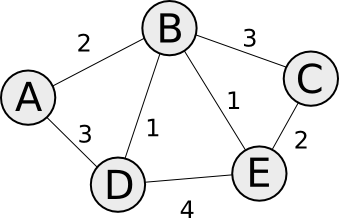
\includegraphics[width=0.5\textwidth]{Graph}
  %   \caption{Weighted graph}
  %   \label{fig:graph}
  % \end{figure}

  %An important factor of a searching algorithm is correctness and also the time required to calculate the optimized path. The algorithms can be rated by their worst-case time, to ensure a responsive performance.

  \subsection{Dijkstra's Algorithm}\label{subs_dijkstra}

  Because every vertex needs to be evaluated the complexity of Dijkstra's algorithm is proportional to the number of vertices.This means that a lot of computational power is required to calculate the result \cite{Dijkstr1959}.

  An example of Dijkstra's algorithm in use is showed in \cref{fig:dijkstra}. Grey blocks are obstacles such as walls. White blocks are unvisited vertices. S marks the start and G the destination. Blue blocks mark vertices that were added to closed set (were visited) and green blocks mark vertices that were added to open set (were considered to be added to closed set). The A marks a point that illustrates that many unnecessary vertices are calculated using Dijkstra's algorithm. B marks a point that shows that Dijkstra's algorithm does consider in which direction the destination is. It keeps searching the graph uninformed until it has visited all vertices in the graph, that is was able to reach from the given source.


  \begin{figure}[ht!]
    \centering
    \frame{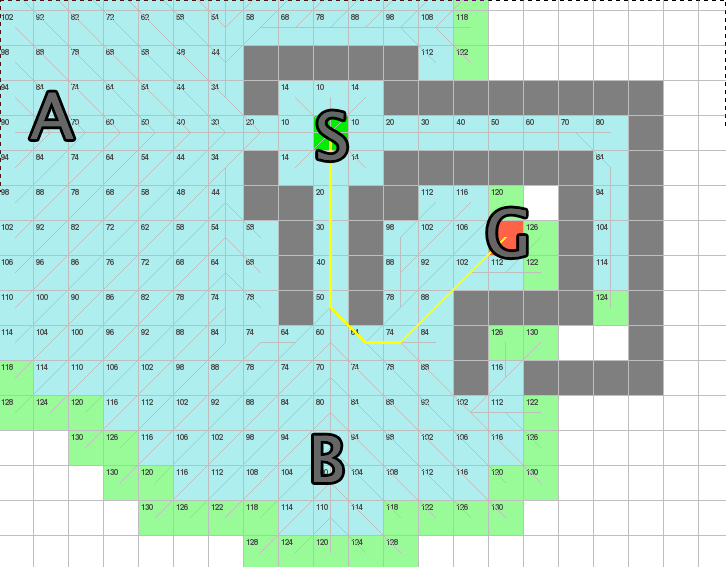
\includegraphics[width=0.5\textwidth]{Dijkstra_edited}}
    \caption{Dijkstra's algorithm in action}
    \label{fig:dijkstra}
  \end{figure}

\subsubsection{Pseudocode}

\Cref{algo:Dij} is a pseudocode example of Dijkstra's algorithm \cite{wiki_dijkstra}. 



\begin{algorithm}
  \caption{Dijkstra's Algorithm}\label{algo:Dij}
  \KwResult{Finds the shortest path from start vertex to vertices}
  \KwData{\\
  graph \tcc*{Graph being searched}
  source \tcc*{The source vertex}
  dist \tcc*{List of distances from source}
  visited \tcc*{List of visited vertices}
  parent \tcc*{List of parents. The parent of a given vertex, is another vertex that provides the shortest current path to the given vertex}
  E-list \tcc*{A list of vertices to be evaluated}
  E-vertex \tcc*{Vertex being evaluated}
  C-vertex \tcc*{Current vertex}
  Temp \tcc*{A temporary variable}
  }

  \SetKwFunction{Dijkstra}{Dijkstra}
  \SetKwProg{KwFn}{Function}{}{}

  \KwFn{\Dijkstra{Graph, source}}{

    \For{\textbf{each} Vertex v in graph}{
      dist[E-vertex] $= \infty$\tcc*{Assign distance from source to as infinite}
      visited[E-vertex] $=$ false\tcc*{Boolean to false for not visited}
      parent[E-vertex] $=$ undefined\tcc*{Assign parent all as undefined}
    }

    dist[$source$] $= 0$\tcc*{Source dist has distance 0}
    insert $source$ in E-list\tcc*{Source dist has distance 0}

    \While{E-list \textbf{is not} empty}{
      C-vertex $=$ E-vertex in E-list with lowest dist[]\tcc*{The new C-vertex is the vertex with lowest dist value}
      remove C-vertex from E-list\tcc*{Remove vertex C-vertex from E-list}
      visited[C-vertex] $=$ true\tcc*{Mark the new vertex C-vertex as visited}

      \For{\textbf{each} neighbour n of C-vertex}{
        $Temp =$ dist[C-vertex] + distBetween(n, C-vertex)\tcc*{Assign temp to the distance from $source$ to C-vertex plus the distance between n and C-vertex}
        \If{$Temp$ < dist[n]}{
          dist[n] $= Temp$\tcc*{Assign $Temp$ as the new shortest distance of vertex n}
          parent[n] $= u$\tcc*{Assign C-vertex as parent of vertex n}
          \If{n \textbf{is not} visited}{
            insert n into E-list\tcc*{Add the unvisited vertex n into the E-list to be evaluated}
          }
        }
      }
    }
    return dist\tcc*{Return the distances in dist}
  }
\end{algorithm}

When Dijkstra's algorithm has been performed, the optimal paths can be induced by backtracking. See \cref{algo:FindPath}.

\begin{algorithm}
  \caption{Find path to target}\label{algo:FindPath}
  \KwResult{Finds the shortest path from start vertex to a target vertex}
  \KwData{\\
        stack \tcc*{Sequence of vertices in path}
        target \tcc*{Evaluating vertex}
        source \tcc*{Source vertex}
        parent \tcc*{A list of parents}
   }

  \SetKwFunction{FindPath}{FindPath}
  \SetKwProg{KwFn}{Function}{}{}

  \KwFn{\FindPath{parent, source, target}}{
    $stack =$ empty sequence\;
    \While{parent[target] \textbf{is not} source}{
      insert $u$ in stack\tcc*{Insert u vertex in the stack}
      target $=$ parent[target]\tcc*{Traverse from target to source}
    }
    return $stack$
  }
\end{algorithm}

\subsubsection{An example of Dijkstra's algorithm in use}\label{subss_dij_ex}

The following steps explains how Dijkstra's algorithm is executed. The example graph is \cref{fig:graph}.

  \begin{figure}[ht!]
    \centering
    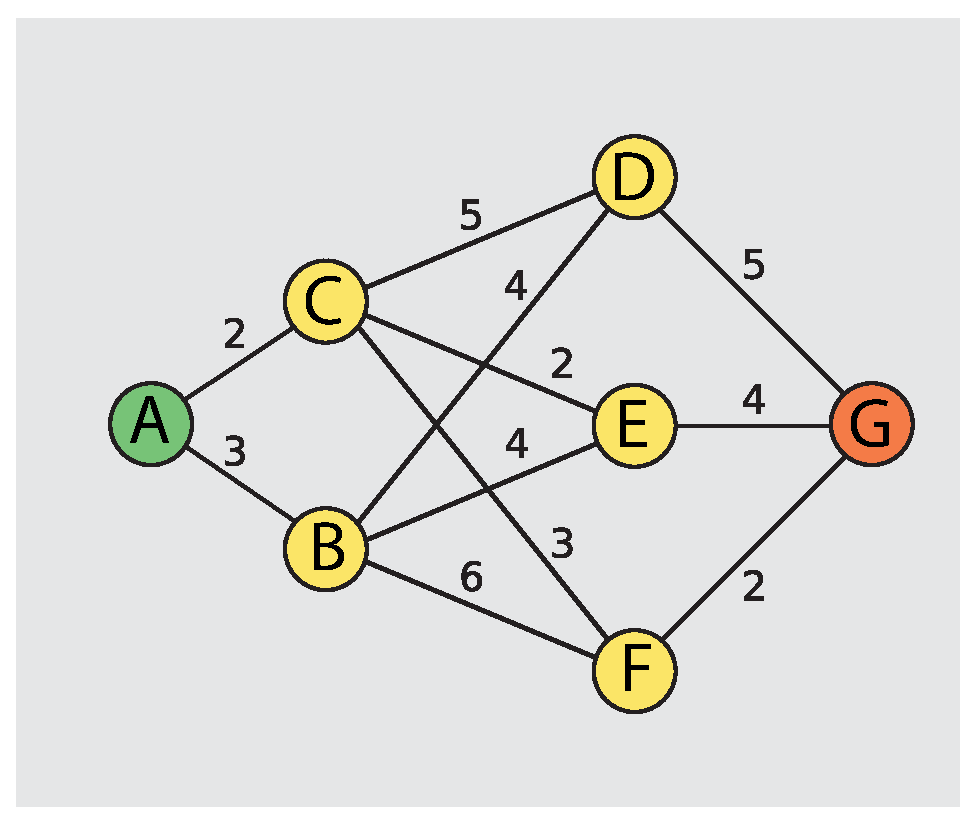
\includegraphics[width=0.5\textwidth]{eksempel_graf.eps}
    \caption{The example graph}
    \label{fig:dij_example_graph}
  \end{figure}

  \paragraph{Step 1}
Set the temporary distance of every vertex in the graph to infinity. The starting vertex should however be set to zero. See \cref{fig:dij_step1}.

  \begin{figure}[ht!]
    \centering
    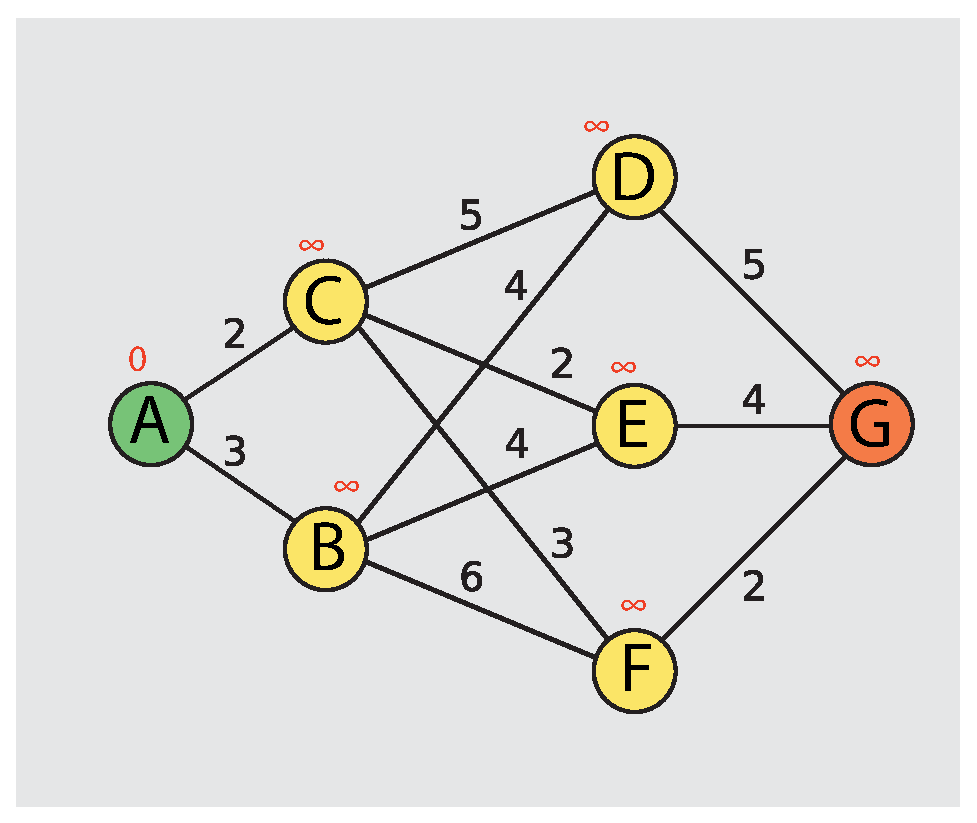
\includegraphics[width=0.5\textwidth]{dij_step1.eps}
    \caption{Step 1 of Dijkstra}
    \label{fig:dij_step1}
  \end{figure}

    \paragraph{Step 2}
Add every vertex to a set called unvisited vertices. Mark the starting vertex as current.

    \paragraph{Step 3}\label{par:dij_step3}
Calculate temporary distances for every neighbour of the current vertex. This is done by adding the distance of the current vertex and the weight of the edge connecting it to the neighbour. See \cref{fig:dij_step2-3}.

  \begin{figure}[ht!]
    \centering
    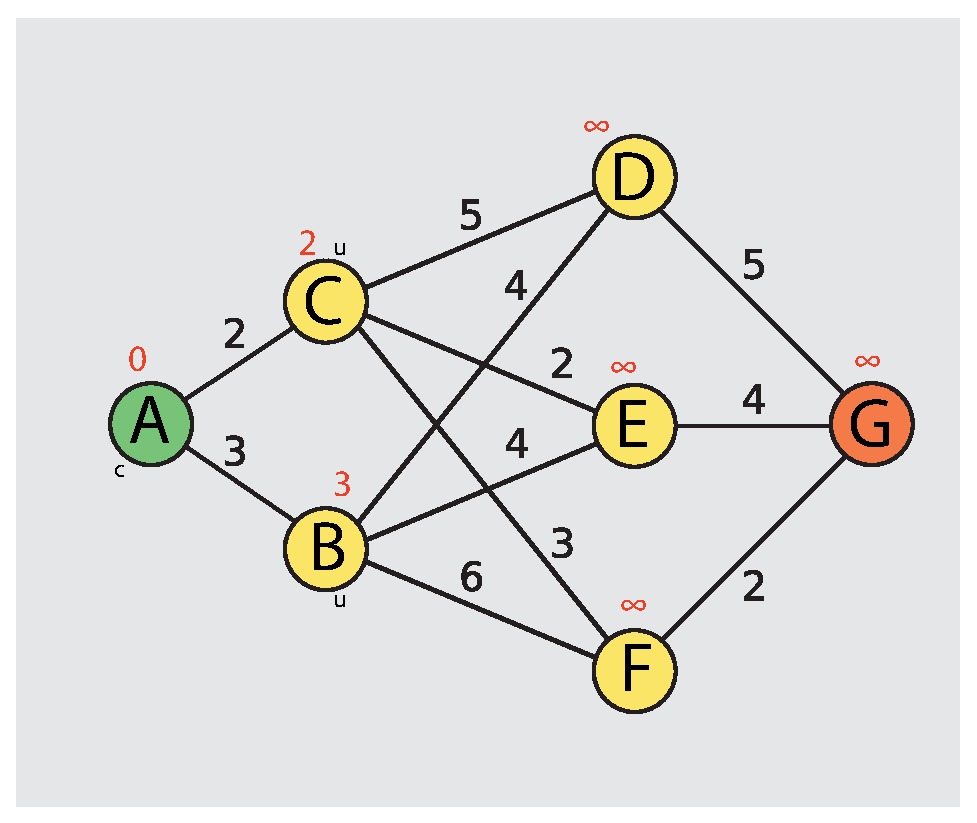
\includegraphics[width=0.5\textwidth]{dij_step2-3.eps}
    \caption{Step 2 \& 3 of Dijkstra. c marks the current vertex. u marks unvisited vertices.}
    \label{fig:dij_step2-3}
  \end{figure}

      \paragraph{Step 4}
When all neighbours have been considered, mark the current vertex as visited, thereby removing it from the set unvisited vertices. This visited vertex will then never be checked again. 

\paragraph{Step 5}
If all vertices have been marked visited or the smallest temporary distance in the unvisited vertices set is infinity, stop the algorithm. The smallest temporary distance in the unvisited vertices set should only be infinity if there is no connecting from starting vertex to destination vertex.

\paragraph{Step 6}
From the unvisited vertices set, select the vertex with the smallest temporary vertex as the current vertex. Repeat step 3 and onwards. See \cref{fig:dij_step4-5-6}.

  \begin{figure}[ht!]
    \centering
    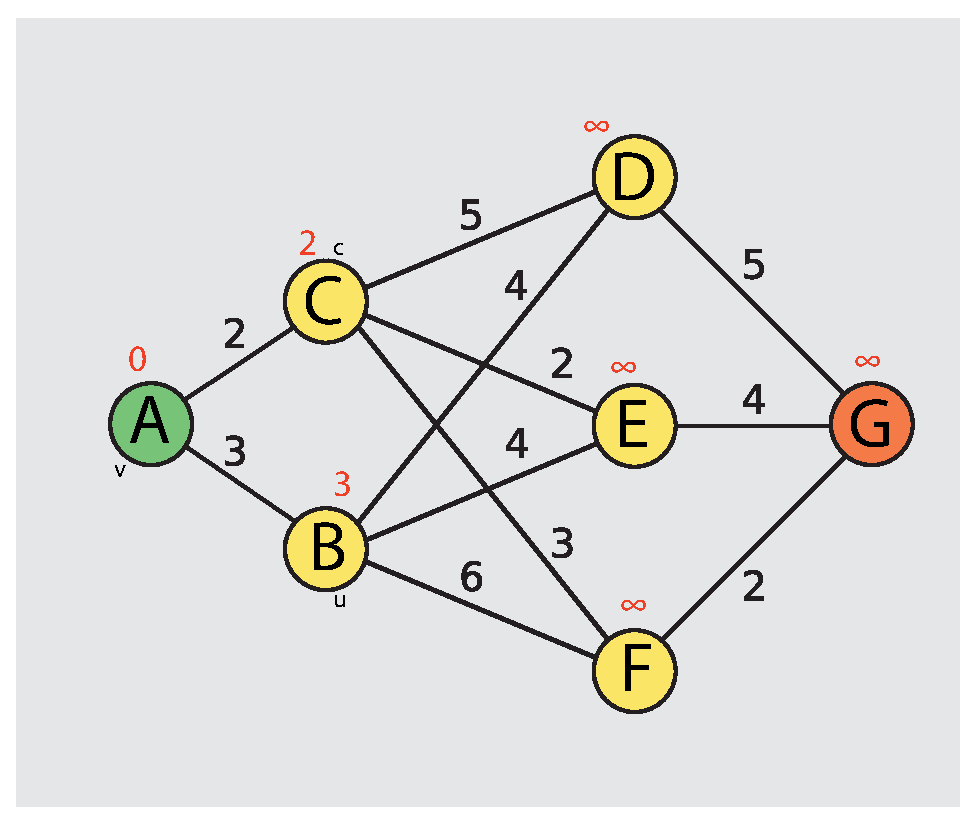
\includegraphics[width=0.5\textwidth]{dij_step4-5-6.eps}
    \caption{Step 4, 5 \& 6 of Dijkstra. c marks the current vertex. u marks unvisited vertices.}
    \label{fig:dij_step4-5-6}
  \end{figure}


  \subsection{A* Algorithm}\label{subs_astar}


  The A* algorithm is an extension of Dijkstra's algorithm providing better performance in terms of speed, while still maintaining the correctness of Dijkstra's algorithm, given an admissible heuristic value. An admissible heuristic value is explained below.

 
  \subsubsection{Heuristic value and evaluation value}
  A* introduces a heuristic value, which is an estimation of total cost from the source to the destination. For it to be admissible, the heuristic value must be exactly equal to or lower than the actual total cost from the source to the destination. If the heuristic value overestimates the cost, A* is not guaranteed to find the shortest path. The lower the heuristic value is compared to the cost value, the less influential the heuristic value is. If the heuristic value is completely without influence, A* performs like Dijkstra's algorithm.

  There are many different methods used to find a heuristic. Two commonly used methods are the Manhattan method and the Euclidean method. These methods typically calculates its results on coordinates. This means that the vertices passed to these methods has to have coordinates describing how the vertices are positioned relative to each other.

    \paragraph{Euclidean distance}\cite{wiki_euclidean}

  \[
    dist(p, q) = dist(q, p) = \sqrt{(q_{1} - p_{1})^2 + (q_{2} - p_{2})^2 + \dots + (q_{n} - p_{n})^2}
  \]

  Where $p$ and $q$ both are vertices in a graph. $p_{n}$ and $q_{n}$ are the coordinates of each vertices. For example $p_{1}$ is the $x$ coordinate of vertex $p$.

    \paragraph{Manhattan distance}\cite{wiki_manhattan_distance}

  \[
    dist(p, q) = dist(q, p) = \| \mathbf{p} - \mathbf{q} \| = \sum\limits_{i=1}^n | \mathbf{p_{i}} - \mathbf{q_{i}} |
  \]

  Where $p$ and $q$ both are vertices in a graph. $p_{n}$ and $q_{n}$ are the coordinates of each vertices. For example $p_{1}$ is the $x$ coordinate of vertex $p$.


  The heuristic value is used to determine the evaluation value. The evaluation value is found by adding the cost from the start vertex to the vertex being evaluated, to the heuristic value. The cost is the total sum of weights of edges visited to the vertex being evaluated. The evaluation value is used when determining if a vertex is in the shortest path. When comparing two vertices, the vertex with the lowest evaluation value is always chosen for the shortest path \cite{Patel2013}.


  For an example of an A* calculation, see \cref{fig:astar}. 
  Grey blocks are obstacles such as walls. White blocks are unvisited vertices. S marks the start and G the goal. Blue blocks mark vertices that were added to closed set (were visited) and green blocks mark vertices that were added to open set (were considered to be added to closed set). A marks a point where the heuristic value increases because the distance to G increases, causing the evaluation value to rise above the threshold for when A* considers another path. Point B marks a point where A* chooses a path around an obstacle.

    \begin{figure}[ht!]
    \centering
    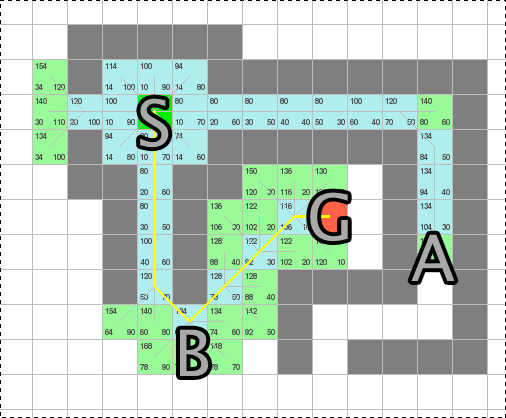
\includegraphics[width=0.5\textwidth]{AstarHlow_kopi.png}
    \caption{Example on an A* algorithm algorithm}
    \label{fig:astar}
  \end{figure}



  % If you would combine Dijkstra's algorithm with Best-First-Search algorithm, you would get the A* algorithm which also utilises the principle of a heuristic estimation to determine which vertex to test next. It uses a evaluation function $f(x) = g(x) + h(x)$, where $g(x)$ describes the cost from the start to the vertex being evaluated, and $h(x)$ is a heuristic function that estimates the cost from the evaluating vertex to the target vertex. \cite{Patel2013}

%\kanote{A WILD DESCRIPTION APPEARS! (referer!)}

\subsubsection{Pseudocode}

A* works by maintaining a priority queue of vertices that need to be examined. This is called the open set. The lower the evaluation value of a vertex is, the higher the priority in the open set. The current vertex is chosen as the vertex with the highest priority in the open set. This vertex is then removed from the open set and its neighbours' evaluation and closedSet values are updated. The neighbor's parent is marked as the current vertex. These neighbours are then added to the open set. The algorithm stops when either the open set is empty or the goal vertex has a lower evaluation value than any other vertex in the open set. If this happens the shortest path to the goal vertex has been found.

The shortest path is then backtracked by starting from the goal vertex and then traversing the goal's parent until the start vertex has been met. These vertices mark the shortest path.

\begin{algorithm} 
  \caption{A* Algorithm}\label{algo:A*}
  \KwResult{Finds the shortest path from start vertex to goal vertex}
  \KwData{ \\
    source  \tcc*{The source vertex} 
    goal \tcc*{The desired destination vertex} 
    closedSet = \{ \} \tcc*{Set of visited vertices} 
    openSet = \{ \} \tcc*{The set of vertices to be evaluated} 
    cameFrom = \{ \} \tcc*{List of navigated vertices} 
    gScore[] = \tcc*{Array containing the cost value for every vertex} 
    fScore[] = \tcc*{Array containing the evaluation value for every vertex} 
    current = \tcc*{Current vertex being evaluated} 
    neighbourVertices(vertex) = \tcc*{Set of neighbours for every vertex}
    hEstimate(vertex1,vertex2) \tcc*{Function that calculates heuristic value}
    distBetween(vertex1,vertex2) \tcc*{Gets cost from vertex1 to vertex2}
    }

  \SetKwFunction{Astar}{Astar}
  \SetKwProg{KwFn}{Function}{}{}

  \KwFn{\Astar{start, goal}}{

    gScore[start] $\gets 0$ \tcc*{Set cost from start to 0}

    fScore[start] $\gets $ gScore[start] $+$ hEstimate(start,goal) \tcc*{Set f value of start vertex}

    add start to openSet\;

    \While{openSet \textbf{is not} empty}{
      current $\gets$ vertex in openSet having the lowest fScore value\;
      
      \If{current $=$ goal}{ 


        return reconstructPath(cameFrom, goal) \tcc*{Goal is reached so reconstruct path and return it}
        }
      }
    
    
    remove current from openSet\;
    add current to closedSet\;

    \For{\textbf{each} neighbour in neighbourVertices(current)}{
      tempGScore $\gets$ gScore[current] + distBetween(current,neighbour)\;

      tempFScore $\gets$ tempGScore + hEstimate(neighbour,goal)\;

      \If{neighbour in closedSet and tempFScore $>=$ fScore[neighbour]}{
        continue \tcc*{Go to the start of the loop, evaluating the next neighbour}
      }

      \If{Neighbour not in openSet or tempFScore $<$ fScore[neighbour]}{
        cameFrom[neighbour] $\gets$ current\;
        gScore[neighbour] $\gets$ tempGScore\;
        fScore[neighbour] $\gets$ tempFScore\;
        \If{neighbour not in openSet}{
          add neighbour to openSet\;
        }
      }
    }

return failure\tcc*{If this point is reached, the goal vertex is never reached}
  }

\end{algorithm}

\begin{algorithm} \label{algo:reconstructPath}
  \caption{Reconstruct path}
  \KwResult{reconstructs the shortest path from start vertex to a target vertex}
  \KwData{\\
        currentVertex \tcc*{The currentVertex being checked}
        cameFrom \tcc*{The vertex currentVertex came from}
        path \tcc*{The path containing the reconstructed path}
   }

  \SetKwFunction{ReconstructPath}{ReconstructPath}
  \SetKwProg{KwFn}{Function}{}{}

  \KwFn{\ReconstructPath{cameFrom, currentVertex}}{

    \tcc{If currentVertex has a parent in cameFrom, call reconstructPath recursively and return the path from reconstructPath + the current vertex}
    \If{CurrentVertex in cameFrom}{
      path $\gets$ reconstructPath(cameFrom, cameFrom[currentVertex])\;
      return (path $+$ currentVertex)\;
    }
    \tcc{CurrentVertex is not in cameFrom list, so no action other than returning currentVertex should happen}
    \Else{
      return currentVertex\;
    }
  }
\end{algorithm}




  % There are multiple ways to calculate the heuristic value(estimated cost) to the target vertex, but an ideal choice would be the Euclidean \cref{equation:Euclidean} distance, as no path can be shorter than the direct distance between two vertices.
  % \begin{equation} \label{equation:Euclidean}
  %   dist((x, y), (a, b)) = \sqrt{(x - a)^2 + (y - b)^2}
  % \end{equation}

  \subsubsection{An example of A* algorithm in use}

  The only notable difference between Dijkstra's algorithm and A* is the use of a heuristic value. The steps 1-6 from \cref{subss_dij_ex} are nearly identical. In step 3 in \cref{subs_dijkstra}, the evaluation value is calculated instead of just the distance.  See \cref{fig:astar_h_explained}.

    \begin{figure}[ht!]
    \centering
    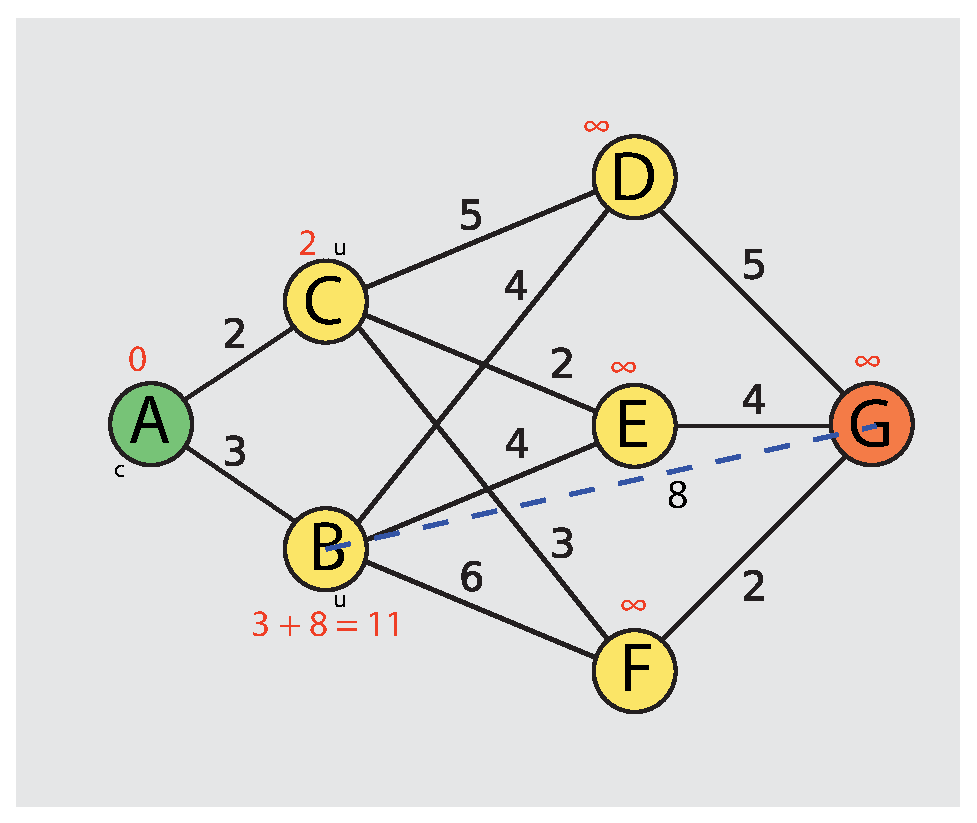
\includegraphics[width=0.5\textwidth]{astar_explained.eps}
    \caption{A*: how is the heuristic value estimated. The dashed line represents the line-of-sight distance.}
    \label{fig:astar_h_explained}
  \end{figure}

  \subsection{Summary of Algorithms}

  There are different kinds of pathfinding problems. These include SSSP and SPSP problems. Dijkstra's algorithm solves SSSP problems and the A* algorithm solves SPSP problems. Dijkstra and A* each have different assets. These are summarized in \cref{tbl:scheme}.
  
  \begin{table}[ht!]
    \centering
  \rowcolors{1}{}{lightgray}
    \begin{tabular}{|r|l|c|}

      \hline
      \textbf{Algorithm} & \textbf{Advantages} & \textbf{Disadvantages} \\
      \hline
      Dijkstra's & Always optimal path & Slow calculation \\
      A* & Optimal path if $h(x)<g(x)$, Fast calculation & Not always optimal path \\
      \hline
    \end{tabular}
    \caption{Table of advantages/disadvantages of different algorithms}
    \label{tbl:scheme}
  \end{table}
